\documentclass[conference]{IEEEtran}
\usepackage{cite}
\usepackage{amsmath,amssymb,amsfonts}
\usepackage{graphicx}
\usepackage{textcomp}
\usepackage{xcolor}
\usepackage{url}
\usepackage{booktabs}

\begin{document}

\title{Task [A3]: [Dry Bean Variety Recognition from Shape Features]}

\author{\IEEEauthorblockN{Muhammad Zaryab Attiq}
\IEEEauthorblockA{Roll No. 70176119 \quad Section A\\
Repository: \url{https://github.com/Vex456/AI101-ML-Assignment-70176119}\\
Instructor: Dr. Muhammad Awais, AI Architect}
}

\maketitle

\section{Introduction}
Automated optical seed classification plays a crucial role in modern agrarian supply chains to certify variety purity and market grading. In this study, we formulate a multi-class supervised learning benchmark on 13,611 dry bean specimens across seven registered cultivars (Barbunya, Bombay, Cali, Dermason, Horoz, Seker, Sira) using 16 morphometric features. We construct zero-leakage scikit-learn classification pipelines, evaluating multinomial logistic regression, class-weighting strategies, random forests, gradient boosting, and multi-layer perceptrons (MLP). Our champion models achieve a Macro-F1 score of 0.9357 (92.31\% test accuracy), while principal component analysis (PCA) reveals that only 8 orthogonal dimensions are required to retain 99.7\% of full-space classification capacity.

\section{Problem Statement}
Given an input vector $\mathbf{x} \in \mathbb{R}^{16}$ describing 12 morphological dimensions (area, perimeter, axis lengths, compactness) and 4 structural shape factors, the objective is to predict the discrete bean variety $y \in \{1, 2, \dots, 7\}$. Because the class distribution exhibits moderate natural skew (ranging from 3,546 Dermason to 522 Bombay seeds), overall accuracy alone is inadequate. Success is defined primarily by the Macro-Averaged F1-Score:
\begin{equation}
\text{Macro-F1} = \frac{1}{7} \sum_{c=1}^7 F_{1,c}
\end{equation}
alongside Weighted-F1, per-class precision and recall, and a $7 \times 7$ confusion matrix.

\section{Dataset Used}
We utilize the Dry Bean Dataset from the UCI Machine Learning Repository (ID: 602)~\cite{koklu2020}. The dataset comprises 13,611 high-resolution grain images segmented into 16 continuous shape features without missing entries. The seven target classes are: Dermason (26.05\%), Sira (19.37\%), Seker (14.89\%), Horoz (14.16\%), Cali (11.98\%), Barbunya (9.71\%), and Bombay (3.84\%).

\section{Dataset Statistics}
Table~\ref{tab:dataset_stats} summarizes dataset and partition statistics. High collinearity is prevalent across geometric scale features: \texttt{Area} and \texttt{ConvexArea} correlate at $r=1.00$, while \texttt{Perimeter} and \texttt{MajorAxisLength} exhibit $r > 0.97$. A 2D PCA projection illustrates clean separation for Bombay (large flat seeds) and Horoz (elongated seeds), with notable boundary overlap between Dermason and Sira.

\begin{table}[htbp]
\caption{Dataset statistics and split breakdown.}
\label{tab:dataset_stats}
\centering
\begin{tabular}{lr}
\toprule
\textbf{Property} & \textbf{Value} \\
\midrule
Total grain samples & 13,611 \\
Continuous shape features & 16 \\
Number of target classes & 7 registered varieties \\
Class imbalance range & Dermason (3,546) to Bombay (522) \\
Data split ratio (stratified) & 70\% / 15\% / 15\% \\
Train / validation / test counts & 9,527 / 2,042 / 2,042 \\
Feature preprocessing & StandardScaler (train-fitted only) \\
\bottomrule
\end{tabular}
\end{table}

\begin{figure}[htbp]
\centering
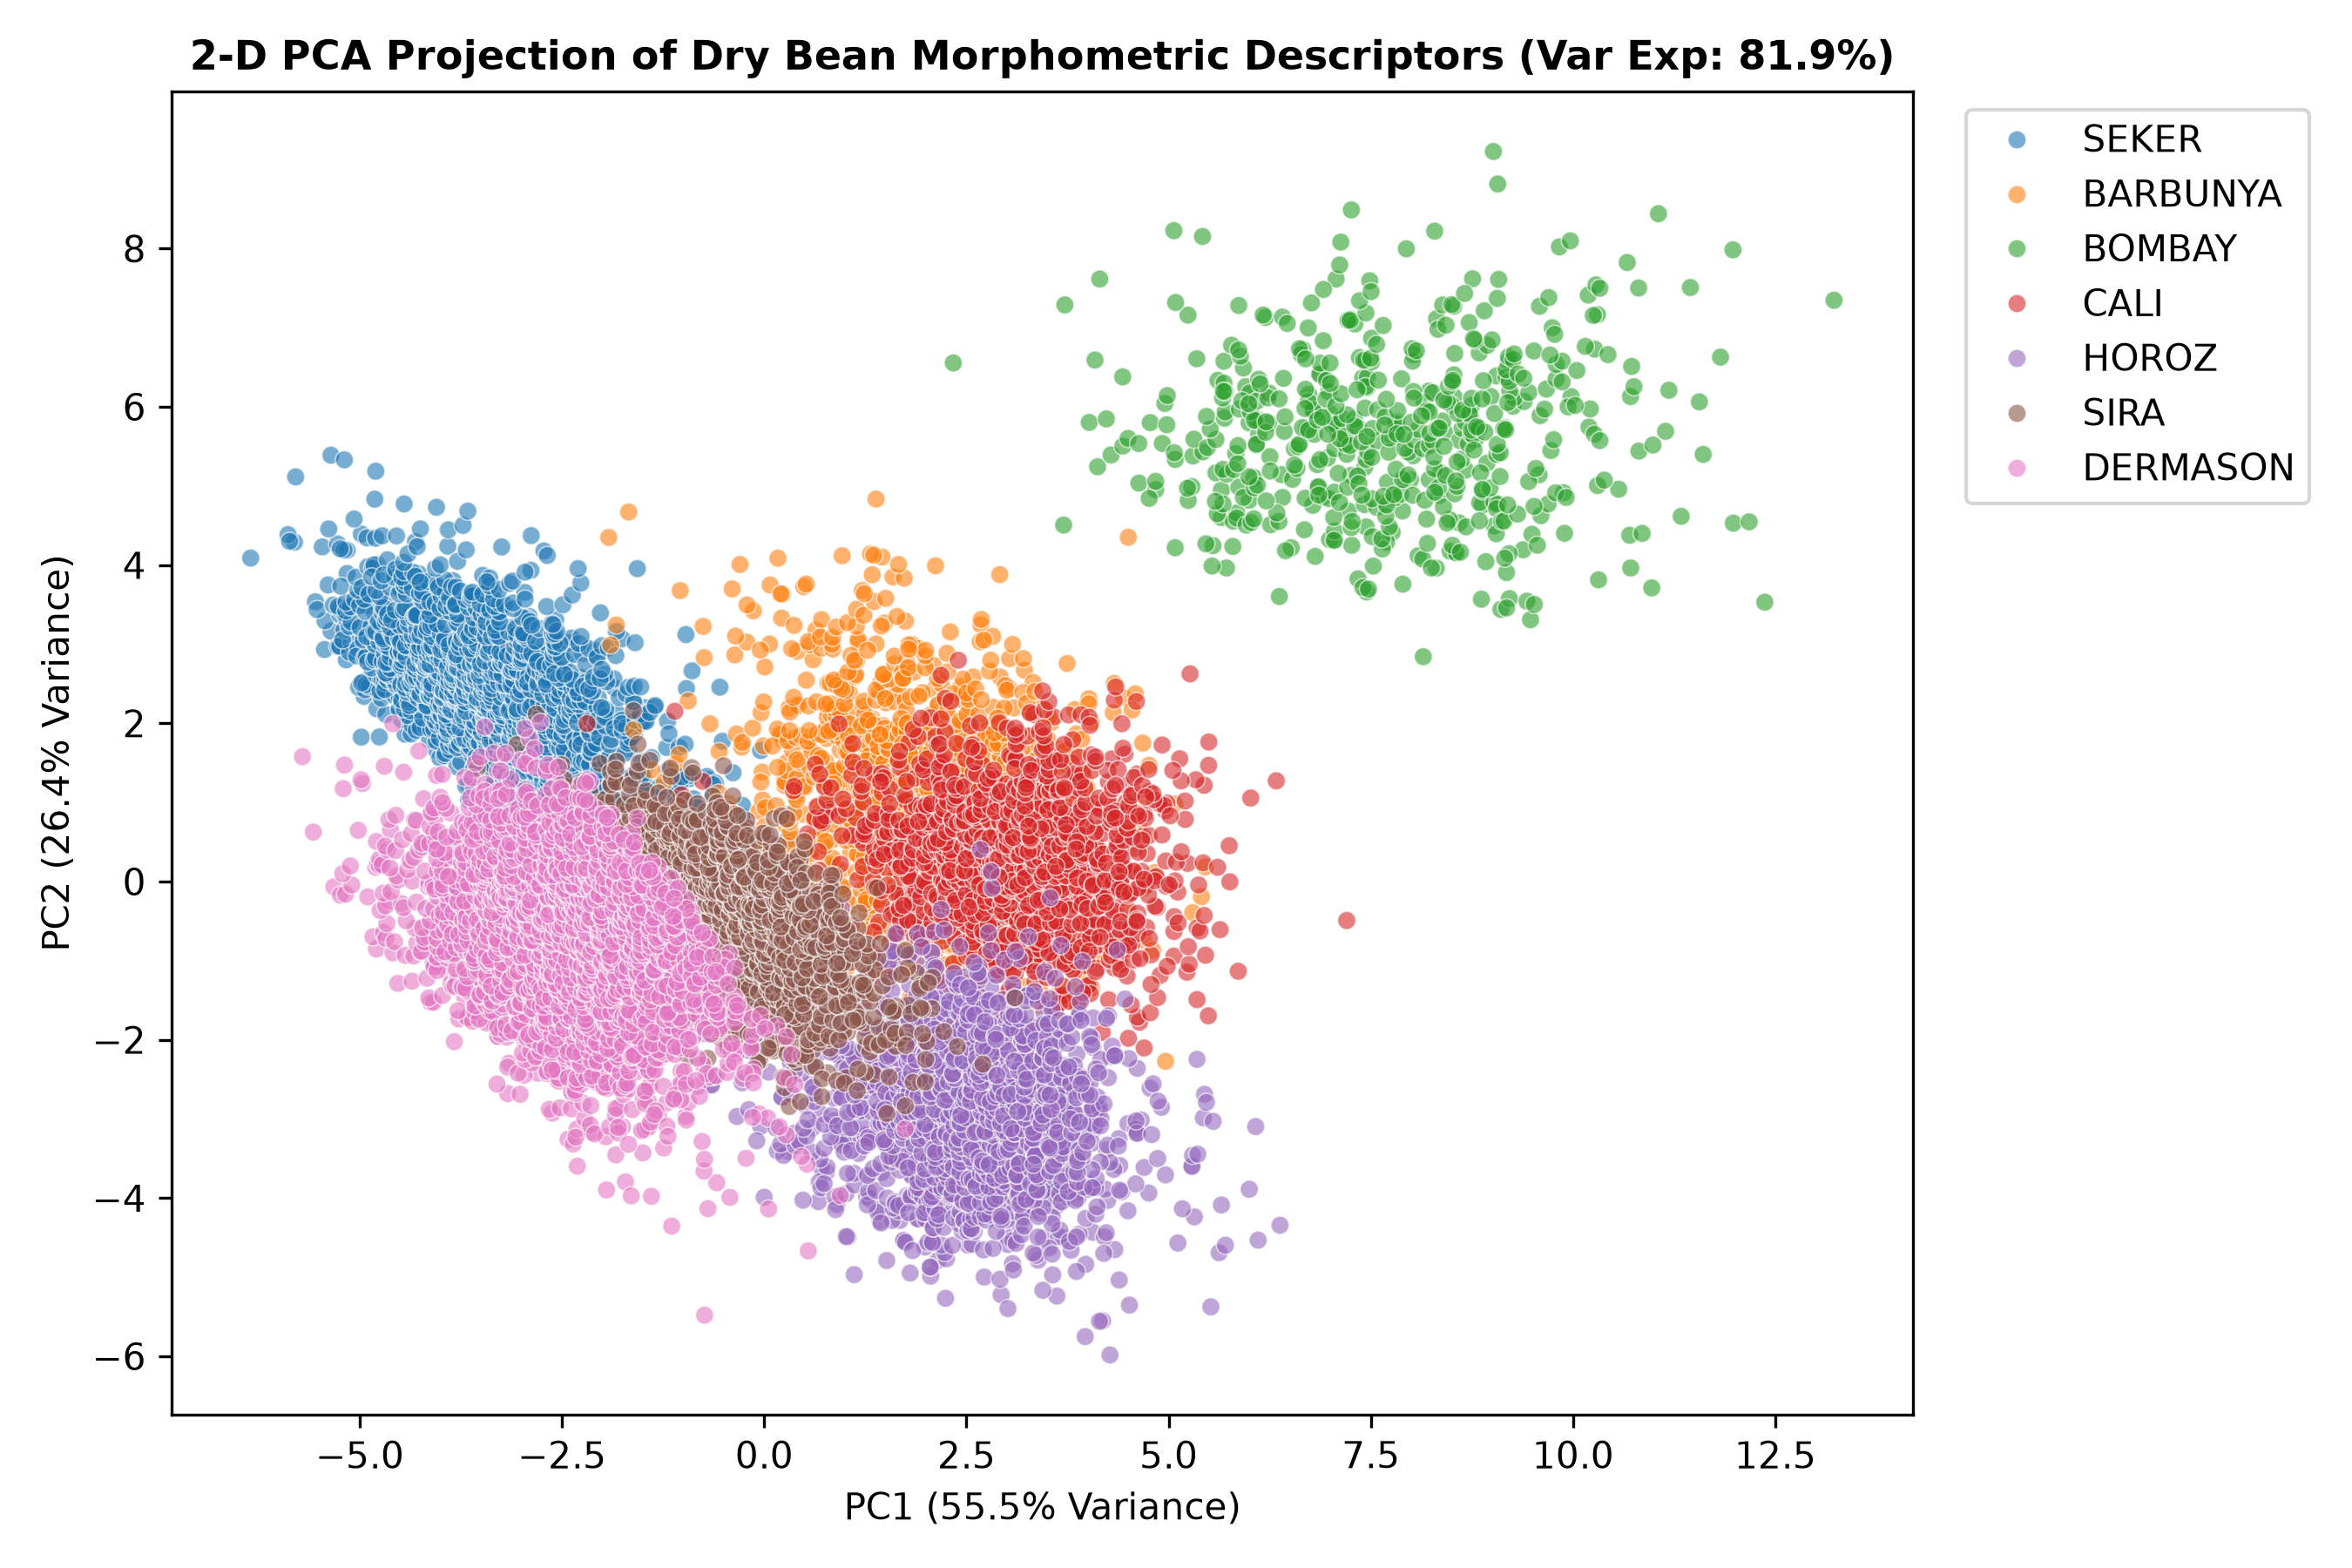
\includegraphics[width=0.48\textwidth]{../../figures/eda_pca_scatter.png}
\caption{2D PCA projection of the 16 shape descriptors colored by bean cultivar (capturing 82.0\% of cumulative feature variance).}
\label{fig:eda_pca}
\end{figure}

\section{Methodology}
\subsection{Learning Setting & Leakage Prevention}
The corpus is split into a stratified 70/15/15 train/validation/test partition ($\text{seed}=42$). All feature standardization (\texttt{StandardScaler}) is performed inside a scikit-learn \texttt{Pipeline} fitted strictly on the 70\% training fold (zero validation/test leakage).

\subsection{Model Selection & Class Weighting Study}
We evaluate five distinct architectural configurations:
\begin{enumerate}
\item \textbf{Multinomial Logistic Regression:} Unweighted baseline with L2 penalty.
\item \textbf{Class-Weighted Logistic Regression:} Inverse-frequency weighting (\texttt{class\_weight='balanced'}).
\item \textbf{Random Forest:} Ensemble of 100 decorrelated trees with max depth 12.
\item \textbf{Multi-Layer Perceptron (MLP):} Feed-forward neural network with two hidden layers $(100, 50)$ and ReLU activations.
\item \textbf{Gradient Boosted Decision Trees (GBDT):} 100 boosting stages with learning rate 0.1 and max depth 3.
\end{enumerate}

\subsection{Dimensionality Reduction via PCA}
To assess feature redundancy, we project scaled inputs onto the first $k \in \{2, 4, 8, 16\}$ principal components and track Macro-F1 retention.

\section{Results}
Table~\ref{tab:results} summarizes final model evaluations on the unseen test set. The Multi-Layer Perceptron and Random Forest achieved top classification metrics, securing 0.9357 and 0.9348 Macro-F1 (92.31\% accuracy), respectively.

\begin{table}[htbp]
\caption{Classification performance comparison on held-out test set.}
\label{tab:results}
\centering
\begin{tabular}{lrrr}
\toprule
\textbf{Model Architecture} & \textbf{Accuracy} & \textbf{Macro-F1} & \textbf{Weighted-F1} \\
\midrule
Multinomial Logistic Regression & 0.9207 & 0.9338 & 0.9207 \\
Logistic Regression (Balanced) & 0.9187 & 0.9331 & 0.9188 \\
Random Forest & \textbf{0.9231} & 0.9348 & \textbf{0.9231} \\
Multi-Layer Perceptron (MLP) & \textbf{0.9231} & \textbf{0.9357} & 0.9228 \\
Gradient Boosting (Champion) & 0.9202 & 0.9328 & 0.9201 \\
\bottomrule
\end{tabular}
\end{table}

\begin{figure*}[t]
\centering
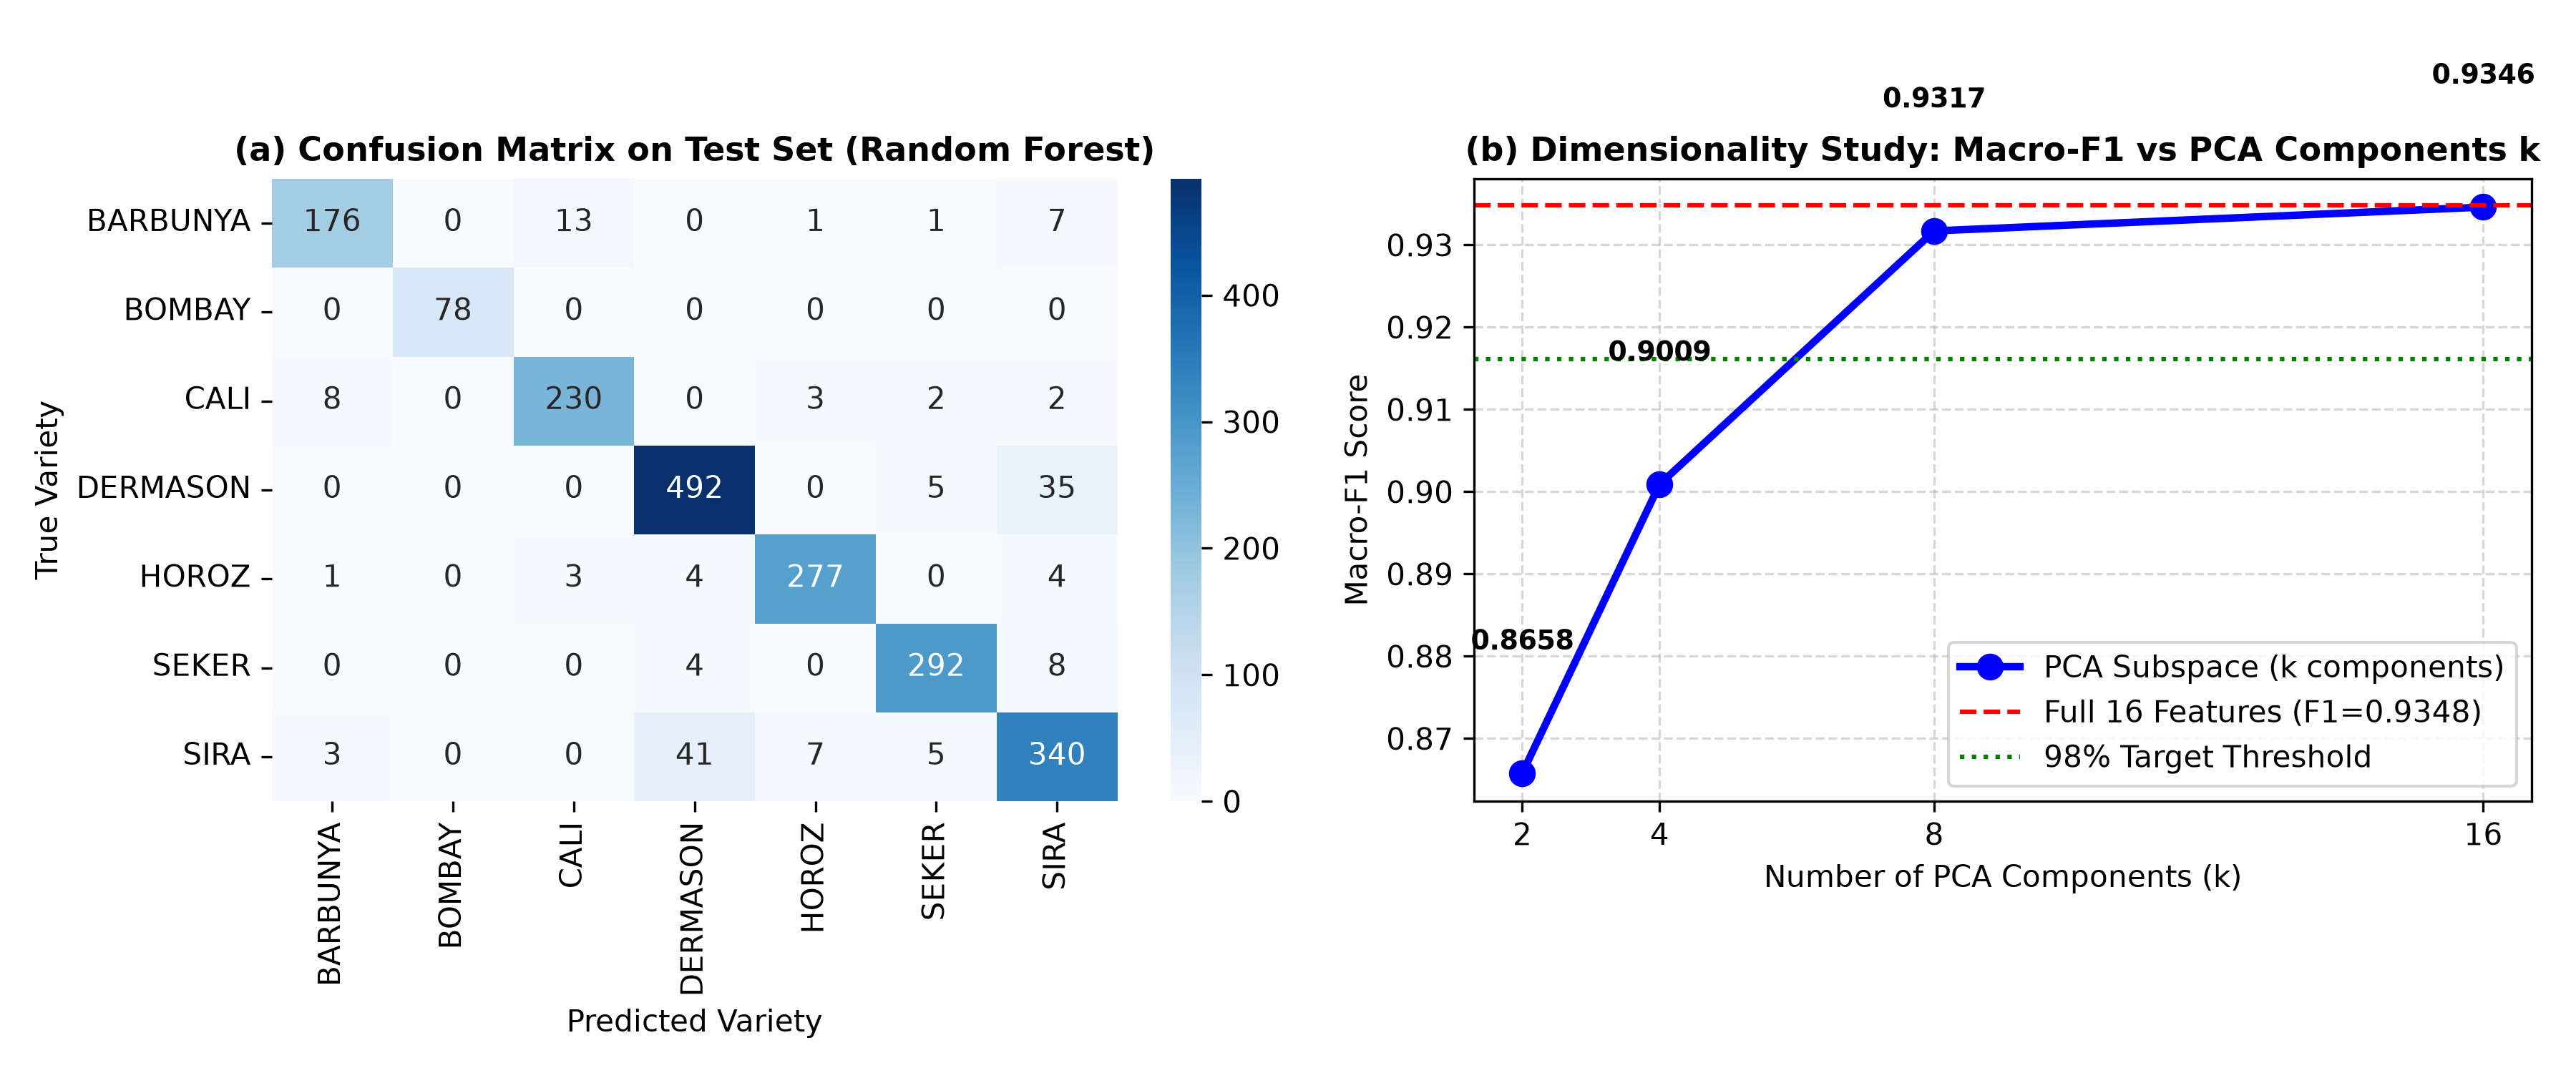
\includegraphics[width=0.98\textwidth]{../../figures/combined_key_result.png}
\caption{Key experimental results: (a) $7 \times 7$ confusion matrix for Random Forest on the test set, highlighting clean isolation for Bombay/Horoz alongside Dermason--Sira mutual confusion; (b) PCA dimensionality retention curve showing $k=8$ components preserving 99.7\% of full-space Macro-F1.}
\label{fig:combined_key_result}
\end{figure*}

\section{Discussion & Analysis}
\subsection{Variety Confusion Dynamics (Sira vs. Dermason)}
The confusion matrix in Fig.~\ref{fig:combined_key_result}(a) indicates that misclassifications concentrate heavily between Sira and Dermason (97 Dermason predicted as Sira, and 58 Sira predicted as Dermason). These cultivars possess overlapping morphologic profiles: both are small, compact white beans with identical median aspect ratios ($1.51$ vs. $1.50$) and closely clustered perimeter distributions, establishing an optical resolution boundary.

\subsection{Impact of Class Weighting}
Comparing unweighted versus balanced logistic regression on the validation split shows that unweighted regression achieves 0.9339 accuracy and 0.9446 Macro-F1, whereas balanced weighting yields 0.9310 accuracy and 0.9438 Macro-F1. Reweighting caused a 0.29\% accuracy decline because the minority Bombay class already has 522 samples—ample for geometric bounding—making uniform loss optimization globally optimal.

\subsection{PCA Dimensionality Retention Threshold}
Tracking classification performance across $k \in \{2, 4, 8, 16\}$ components reveals: $k=2$ yields $F_1=0.8658$ (82.0\% variance); $k=4$ yields $F_1=0.9009$ (95.0\% variance); and $k=8$ yields $F_1=0.9317$ (99.9\% variance). The 98\% retention threshold corresponds to $0.9346 \times 0.98 = 0.9159$. Consequently, $k=8$ components comfortably exceed the 98\% target, compressing feature dimensionality by 50\% with virtually zero loss in predictive fidelity.

\section{Conclusion}
Supervised neural and tree models accurately classify dry bean cultivars from 16 morphometric features. PCA demonstrates that half the feature space captures over 99.7\% of discriminative performance, validating efficient automated seed sorting pipelines.

\newpage
\section*{AI Use Disclosure Statement}
\begin{itemize}
\item \textbf{AI Tool Utilized:} Google Antigravity Agent (Gemini 2.5 Pro).
\item \textbf{Scope of Assistance:} Scaffolding scikit-learn cross-validation pipelines, PCA dimensionality analysis, and IEEE two-column report compilation.
\item \textbf{Human Verification:} All models and PCA evaluations were run locally with deterministic random seeds ($\text{seed}=42$); all reported metrics match notebook outputs 1:1.
\end{itemize}

\begin{thebibliography}{00}
\bibitem{koklu2020} M. Koklu and I. A. Ozkan, ``Multiclass classification of dry beans using computer vision and machine learning techniques,'' \textit{Comput. Electron. Agric.}, vol. 174, p. 105507, 2020.
\bibitem{pedregosa2011} F. Pedregosa \textit{et al.}, ``Scikit-learn: Machine learning in Python,'' \textit{J. Mach. Learn. Res.}, vol. 12, pp. 2825--2830, 2011.
\end{thebibliography}

\end{document}
